\documentclass[]{final_report}
\usepackage{graphicx}
\usepackage{hyperref}
\usepackage{fix-cm}

%%%%%%%%%%%%%%%%%%%%%%
%%% Input project details
\def\studentname{Terique Carnegie}
\def\reportyear{2024}
\def\projecttitle{Playing Games and Solving Puzzles Using Artificial Intelligence}
\def\supervisorname{Michail Fasoulakis}
\def\degree{BSc (Hons) in Computer Science}
\def\fullOrHalfUnit{Full Unit} % indicate if you are doing the project as a Full Unit or Half Unit
\def\finalOrInterim{Interim Report} % indicate if this document is your Final Report or Interim Report

\begin{document}

\maketitle

%%%%%%%%%%%%%%%%%%%%%%
%%% Declaration

\chapter*{Declaration}

This report has been prepared on the basis of my own work. Where other published and unpublished source materials have been used, these have been acknowledged.

\vskip3em

Word Count: 5,186

\vskip3em

Student Name: \studentname

\vskip3em

Date of Submission: 13/12/2024

\vskip3em

Signature: \studentname

\newpage

%%%%%%%%%%%%%%%%%%%%%%
%%% Table of Contents
\tableofcontents\pdfbookmark[0]{Table of Contents}{toc}\newpage

%%%%%%%%%%%%%%%%%%%%%%
%%% Your Abstract here

\begin{abstract}

  The general purpose of artificial intelligence is to give computers the ability to replicate human intelligence through the use of problem-solving algorithms. AI has the potential to outperform human intelligence in solving many different and difficult problems due to its ability to “think” by running problem solving computations at much greater speeds and accuracy than a human and it does this through leveraging the superior processing capabilities of a computer~\cite{AIforSocialGood}. 

  Due to the nature of problem-solving algorithms, Artificial Intelligence is able to provide assistance and insight into many different fields of expertise making it popular and very much in demand as an asset to humanity. In order to increase the value of AI, it is necessary to deeply research ways to improve problem solving algorithms and to discover which of the algorithms works best for a specific problem, and it is also important to develop methods for humans and AI to safely interact. One way this can be achieved is through games and puzzles. Using games and puzzles as a means to research and further develop AI can be very beneficial as it allows for problem solving algorithms to be tested against fun solvable challenges which can provide insight on how well the algorithms are able to solve problems, using games can also provide a way for humans to interact with artificial intelligence through either testing the speed and efficiency of both the player and the algorithms or through the use of 2 player games like chess and checkers. This type of approach to using artificial intelligence has been seen in the past from the first working checkers program to appear in 1952~\cite{Kister1957}, and chess playing programs being developed shortly thereafter~\cite{Strachey1952} which had a role in furthering research and development of modern algorithms and uses of Artificial Intelligence. 

\end{abstract}
\newpage

%%%%%%%%%%%%%%%%%%%%%%
%%% Introduction
\chapter{Introduction}

\section{Artificial Intelligence Solving a Sudoku}

Artificial Intelligence has been applied to many different fields of expertise and has had many advancements in their problem solving algorithms. Some of the more modern and complex problem-solving AI algorithms that can be engineered to play and solve challenges in games are backtracking algorithms, constraint satisfaction algorithms, search algorithms, minimax algorithms, Monte Carlo Tree Search, reinforcement learning and neural networks. All of these algorithms allow for AI to be able to play games and potentially interact with human players, however for the sudoku solver, the project will focus on and utilise only a few of these AI algorithms. The selected algorithms for solving this problem will be back tracking and neural network algorithms. The other problem-solving algorithms are capable of providing a solution but my reasonings for my selection will be explained in the following paragraphs.  

There are several different types of backtracking algorithms, such as consistency pruning, looking ahead, efficient backtracking and variable and value heuristics, but the basic principle behind backtracking algorithms is to explore all possible solutions through attempting different paths recursively and regressing back to try a different path when the current is no longer deemed viable. A sudoku can be solved by assigning numbers to an empty square but validating the number before to check if it is safe to assign, however this kind of approach has a worst-case time complexity of $O(9^{n \cdot n})$ \cite{GeeksforGeeks}. 

Neural networks like convolutional neural networks and recurrent neural networks can be used to solve problems through pattern recognition. It does this by imitating how the human brain works through layers of interconnected nodes that takes in data, performs computations on the data and provides a prediction based on the data analysed. This can be applied to solving a sudoku as if trained on the rules and sequences of numbers of sudoku training data, the algorithm could be able to predict the numbers that will fit sudoku sequence with up to 99\% accuracy \cite{AkinDavid}.

\section{Purpose of my Application}

Through this project I plan further the understanding of how Artificial Intelligence can be applied to solve games and puzzles with logical thinking and pattern recognition by developing a platform using the Python programming language for developing my AI algorithms, with the pygame library for the development of the Graphical User interface and the Visual Studio code IDE to effectively manage my work files, to aid in my projects goal of demonstrate the capability of Artificial intelligence and how it can quickly assess and solve puzzles and problems in a gaming environment, by creating multiple problem-solving algorithms which will tackle and solve sudoku puzzles of increasing sizes and complexity, and evaluating which of the following algorithms between both backtracking and neural networks is better  for solving a sudoku puzzle efficiently and potentially faster than humans in most cases. 

\section{Project Milestones}

There were a couple of milestones achieved in the development of the Artificial Intelligence solver. The following milestones played a significant role in putting together the application so that it can run and achieve the goals that the project was set to achieve within the first term of development, these milestones were: 

\begin{itemize} 
    \item \textbf{The development of the Console Interface:} this milestone had significance in the project as this milestone allowed for displaying the puzzle on the screen both solved and unsolved, this was a needed milestone as if the grid could not be displayed to the screen, it would be difficult to develop any of the AI algorithms as determining if the solving algorithms are outputting the correct results as reading from the array is not very efficient or user friendly due to the lack of a grid layout and sub-grid division. 

    \item \textbf{The development of the Backtracking algorithm:} the first solving algorithm is key and very a very important milestone for this project as it displays that AI can be adapted to playing games and solving puzzles, as well as demonstrating how it is able to do so in a much shorter amount of time when compared to humans. However, having only one algorithm to demonstrate this is not optimal, it shows that progress has been made, and that the second term of development can be geared towards the development of a secondary algorithm to further back the claims my project aims to prove. 

    \item \textbf{The development of the Graphical User Interface:} having a graphical user interface to display the steps and speed of the algorithm to a user is beneficial to proving that algorithm can learn from its mistakes, mimicking human intelligence, as it shows the algorithm choosing the incorrect solution and when realising its mistake, is displays the algorithm changing its solution to a valid one. This helps to demonstrate that AI can be used to solve problems quickly through the Sudoku grid solving animations that are run in the pygame window.
\end{itemize}

%%%%%%%%%%%%%%%%%%%%%%
%%% Application Development
\chapter{Application Development}
\section{Development of Terminal Interface}

The main focus for the start of the sudoku solver needs to be the interface for displaying the sudoku. This is a necessary starting point as in order to demonstrate Artificial Intelligence solving the sudoku, the product needs to be able to display both the unsolved and solved solution in a way that is easily digested by the target audience. The borders, regions, numbers and void values need to be distinct and observable to those trying to understand what the AI algorithms is trying to achieve, and if the algorithms are doing so correctly. That makes this element of the product integral to the development of my project. 

The best approach to initially work on this feature would be to work on a console based interface. This would be effective as the first iteration of the sudoku interface as it only needs to display an easily readable representation of the sudoku puzzle. This was achievable in the console as the borders can be represented through the '-' character for row division and '|' character for column division, the numbers as just numbers and the void values as an '*' character. this gave a simple and easy to read sudoku display on the console.

Division of the grid into sub-grids in the terminal would work through calculating the size of the sub-grids which can be based upon the size of the inputted grid as in most cases the length of the sub-grid is the square root of the length of the grid, for example, a 9x9 grid would have 3x3 sub-grids or a 16x16 would have a 4x4 sub-grids. However, in some cases a sudoku can have sub-grids with unequal length rows and columns, such as a 6x6 grid which has 2x3 sub-grids or a 12x12 which has 3x4 sub-grids. For the solver to be able to adapt so that it can print and solve sudokus of different sizes the application would need to be able to work out the correct row and column length based of the grid size. 

A way to approach the interface algorithm is to calculate the square root of the grid length, and storing this value as a row and column divisor, however in the case where the square root is not a whole number, the algorithm rounds the value down for the row divisor and rounds it down for the column divisor but adds 1, which in most cases is enough to find the correct sub-grid lengths, as in the case of a 6x6 grid, the algorithm would calculate the root to 2.449... and round it down to 2 for the row divisor and set the value to 3 for the column divisor, creating the 2x3 sub-grids necessary for displaying the puzzle. 

The divisors would be used by the algorithm to print a series of '-' characters for every row which is fully divisible by the row divisor, which separates the rows in the sub-grids. And for the columns, the algorithm would print the '|' character in the column index which is fully divisible by the column divisor. With this algorithm, the application is capable of taking in sudokus in the form of a 2 dimensional array and displaying a user friendly way of observing both an unsolved and solved sudoku problem. 

A look at the final sudoku printing algorithm:
\begin{verbatim}
  def print_grid(self, grid):
  if(grid == None):
      print("No found solution!")
      return
  divisor = grid.__len__() ** 0.5
  if(divisor%1!=0):
      row_divisor = round(divisor)
      column_divisor = round(divisor)+1
  else: row_divisor, column_divisor = divisor, divisor
  # logic for dividing sudoku grid into regions depending on sudoku length
  for i in range(grid.__len__()):
      if i % row_divisor == 0:
          print(" - "*grid.__len__())
          # uses dividing value to place row borders
      row=""
      for j in range(grid[i].__len__()):
          if(j % column_divisor ==0):
              row+= " |"
              # uses dividing value to place column borders
          row+=" "+str(grid[i][j]) if grid[i][j]!=0 else " *"
          # adds number or * to be printed for final sudoku output
      print(row+" |")
  print(" - "*grid.__len__())
  # printing the numbers of grid list or an * where there is a 0
  # and the borders to display the sudoku in the console to the user
\end{verbatim}

\section{Development of Backtracking Algorithm}
\subsection{What is Backtracking?}

Backtracking is a main method of creating an AI algorithm to solve a constraint satisfaction problem. Constraint satisfaction problems are problems in which there are a finite set of variables that contain a finite domain of potential values which can be assigned to form a solution. These values will need to satisfy all the constraints of the problem in order for it to be a correct answer. Examples of CSPs are scheduling, puzzle solving such as sudokus and even resource allocation. Backtracking is an example of a complete algorithm, in which it can guarantee the if a solution does or does not exist for the constraint satisfactory problem \cite{Brailsford1999}. 

Implementing a backtracking algorithm to solve a CSP is done through recursion and may even use a decision tree in order to represent the different potential values for the variable set of the CSP \cite{vanBeek2006} 
The algorithm would generally work through choosing a value for a variable in the set, validating its choice, and if at any point a valid value for a variable can not be found, it will backtrack to a point were alternative decisions are available and have not all be exhausted and a different path to a potential solution is taken. This is done repeatedly until a solution is found, or there are no longer any unexplored values (all decisions have been exhausted completely) meaning that there is no solution to the constraint satisfaction problem \cite{Melanie2024}. 

\subsection{Implementation of Backtracking Algorithm}

A backtracking algorithm works similar to how a human would use backtracking as once a human discovers a mistake, an approach to fixing it would be to go back on their working out and find the cause of fault which gives them the undesirable output. The algorithms would work by making its own attempt to solve a problem. so in the case of a sudoku it would attempt to fill in blank squares with a potential valid value, and if a problem occurs in its solution later on, such as the next blank square not being able to find a single valid value, then the algorithm would need to progress back to the cause of the problem, which would be the incorrect value in the previous square, or the ones before until it finds a different valid value to progress. The backtracking algorithm will then continue its attempt with a different solution for the sudoku, and this is done repeatedly till a viable solution is formed.  

When developing the solving algorithm, first came the crucial element of finding a blank square in the grid, this would be represented by a 0 in the sudoku grid’s 2 dimensional array. the coordinates on the grid would be returned to the main algorithm when found, then using these, the main loop will attempt to fill the square with numbers ranging from 1 to the max value, which is also the length of the grid (usually 9), until a viable value for the square is found. In order to check the validity of a value, the algorithm would exhaustively search through the row, column and sub-grid (checking every value in that area) for the value that is equal to the value about to be inputted into the blank square if the value is not found in any of the specified areas then it is considered valid, if the same number is found, then the current value is invalid and the algorithm attempts to check  the next value for validity. If a viable value cannot be found, the algorithm clears the current square and backtracks to the previous square, and checks the next values for viability, if there are no viable values, the algorithm will clear the current square and backtrack once again to the square before and once again try different values until a different viable value is found and the algorithm searches for the next blank value and the algorithm repeats itself, until there is no more blank squares, or no more values to try on the grid that gives a solution to the problem. 

A look at the main Backtracking algorithm:
\begin{verbatim}
  def backtracking(grid, sudoku):
    position = empty_space(grid)
    # locates an empty square on the grid and stores its location
    if position == None:
        return grid
        # if there are no empty squares, the solution has been 
        # found and the grid is returned
    for i in range(1, grid.__len__()+1):
        sudoku.update(i, position[0], position[1])
        # updates the GUI to display the current attempt for a viable value
        if safe_value(grid, position, i):
            grid[position[0]][position[1]] = i
            # test a viable number in the open position
            backtracking(grid, sudoku)
            # checks the next space after the previous viable solution
            if(empty_space(grid)==None):
                return grid
                # if the are no empty positions, this solution is correct
        grid[position[0]][position[1]] = 0
        # if the current value is not viable, it is set to 0, but the i remains
        # as the none viable solution to be incremented
        sudoku.update(0, position[0], position[1])
        # updates the GUI to clear the current square
    return None
    # if there is no number that goes into the empty position, 
    # an empty grid is returned as there is no solution
\end{verbatim}

\section{Development of Graphical User Interface}

For the development of the graphical user interface to display the sudoku and the solving algorithm, pygame was a powerful python library to leverage in the programming of the GUI as it provides an adaptable environment in which the sudoku grid can be drawn on the window and updated with little difficulty while still being able to display a way of visualising the backtracking algorithm. When creating the grid on the window it was best to give it the length 340 which was big enough for the user to see the sudoku and the values in each square clearly. When dividing the grid into sub-grids, the same root and rounded divisor logic used in the console print function, however in the case of the GUI the grid was divided visually using thicker lines to create the division between the whole and sub grids. Then after the grid has been drawn in the window, the algorithm starts adding values to square by placing a new square over the empty square with the intended value. 

It is also necessary to be able to clear the squares within the grid, this is so that the sudoku solver will be able to show its iterations of the solution. In the updating squares method, the squares cleared through overwriting the square by filling the surface with a white square then updating the value to a new square to cover the cleared square. this function would need to be called every time the value changed in the algorithm in order to give the visual backtracking effect. 

By introducing a GUI to display the solving algorithm, the solver is able to show the step by step solution being formed through mistake adaptation approach my backtracking algorithm takes as well as showing how quickly the computer can calculate this as the GUI updates the values very rapidly, demonstrating how much faster a computer is compared to a human, despite the GUI technically wasting computer processing speed, so it is faster to print the output directly then updating a GUI, but then the algorithm will not be demonstrated in an easily comprehensible manner when being displayed in that manner. 

The main loop for the displaying the grid in the GUI
\begin{verbatim}
  for row in range(grid.__len__()):
            self.board.append([])
            # adds a array inside another array, representing rows on the board
            if(row%row_divisor==0 and row != 0):
                pygame.draw.line(self.screen, (0, 0, 0), 
                (col_offset, row*square_size), 
                (col_offset+(grid.__len__()*square_size), row*square_size), 8)
                # where the board is divided based on divisor, 
                # thicker lines are used to show the divisions that 
                # make up the sub-grids
            for col in range(grid.__len__()):
                square = pygame.Rect(col_offset+(col*square_size), 
                row*square_size, square_size, square_size)
                value = self.font.render("" if grid[row][col] == 0 
                else str(grid[row][col]), True, (0, 0, 0))
                val_rect = value.get_rect()
                val_rect.center = square.center
                self.screen.blit(value, val_rect)
                self.board[row].append(square)
                pygame.draw.rect(self.screen, (0, 0, 0), square, 1)
                # the squares are created within the boundaries of the grid,
                # and smaller rectangles with the preset
                # puzzle values are displayed within the squares where their 
                # coordinates are found from the input array
                if(col%column_divisor==0 and col != 0):
                    pygame.draw.line(self.screen, (0, 0, 0), 
                    (col_offset+(col*square_size), row*square_size), 
                    (col_offset+(col*square_size), grid.__len__()*square_size), 8)
                # where the board is divided based on divisor, thicker lines are used 
                # to show the divisions that make up the sub-grids
\end{verbatim}

%%%%%%%%%%%%%%%%%%%%%%
%%% Current Progress
\chapter{Current Progress}

\section{Application Architecture}

The project was divided in a way so that each file would have a specific purpose, a specific feature that would be needed to be used by the main file, in which the entire application is ran from. This organisation of the code base is beneficial as it allows for the program to be well documented, as the comments written in a file is relevant and specific to the feature being programmed. Also this architecture is good for the development of classes and features as they can be built upon and tested independently of one another which is necessary for keeping and maintaining good quality code for the AI sudoku solver, this also has the additional benefit of making feature updates and improvements easier to implement as making changes will only affect the current feature code and potential bugs will not be able to interfere with the progress being made on the other features of the main application. 

An agile type of methodology style was implemented in the development process of the AI sudoku solver as the primary focus of the term time development cycle was putting together rapidly developed features that is capable of doing just enough to get the application running and connecting them together to get a working prototype which is able to print and solve the puzzle in a way which is easily interpreted by the applications intended users. This style of development will be carried out in the next term of development also as it would be more important to focus on developing the key features of the application so that the prototype is able to meet the set aims and objectives of the project and only once these are achieved, improvements and updates can be made to the code base to improve the application incrementally until the final product has been formed. 

\section{Running the Application}

When running the main application there 2 different sets of outputs are provided for the user to examine, the console displayed unsolved and solved sudoku puzzle and the pygame window in which the puzzle is displayed initially unsolved, and then shows the step by step procedures the solving algorithm takes to present the user with an actual solution. 

The console based output was beneficial to the first sprint development cycle as it got the job done in terms of displaying what the algorithm needed to solve and the result the AI algorithm produced, this method of output done best at showing just how quickly the AI algorithm could solve the problem as it would almost instantly display both the unsolved and solved solution to the sudoku. However, this method of output was inefficient of displaying the steps and the decisions that the algorithm makes as I would need to print multiple instances of semi-complete solutions, which is not a console friendly design as many iterations and decisions are made, so the mistakes and inaccuracies made before the solution is found is abstracted from the users. 

\begin{figure}[ht]
    \centering 
    \begin{minipage}{0.3\textwidth} 
        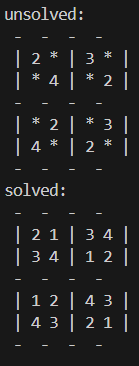
\includegraphics[width=\textwidth]{images/terminal 2x2.png} 
        \caption{2x2 grid} 
        \label{fig: terminal 2x2} 
    \end{minipage} 
    \hfill 
    \begin{minipage}{0.3\textwidth} 
        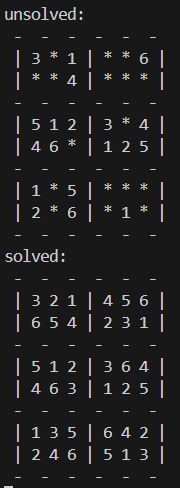
\includegraphics[width=\textwidth]{images/terminal 6x6.png} 
        \caption{6x6 grid} 
        \label{fig: terminal 6x6} 
    \end{minipage} 
    \hfill 
    \begin{minipage}{0.3\textwidth} 
        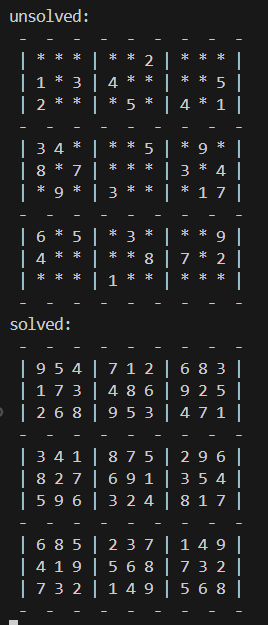
\includegraphics[width=\textwidth]{images/terminal 9x9.png} 
        \caption{9x9 grid} 
        \label{fig:terminal 9x9} 
    \end{minipage}
\end{figure}

\clearpage
The GUI based output was a beneficial for its ability to display the steps and decisions that the algorithm takes to find the solution. It shows the mistakes the algorithm finds and shows the how it works backwards, similarly to how a human would potentially try and find the solution to the sudoku problem. However, this form of output, despite solving the solution fairly quickly, potentially much quicker than most humans could, due to the algorithm requiring extra steps of clearing the squares and updating its value on the window’s grid means that this output is generally slower as more computational power is needed from the machine, although this is not that serious of an issue as the speed of the solving algorithm is still capable of proving and meeting the aims and objectives the application was set out to achieve. 

\begin{figure}[ht]
    \centering 
    \begin{minipage}{0.3\textwidth} 
        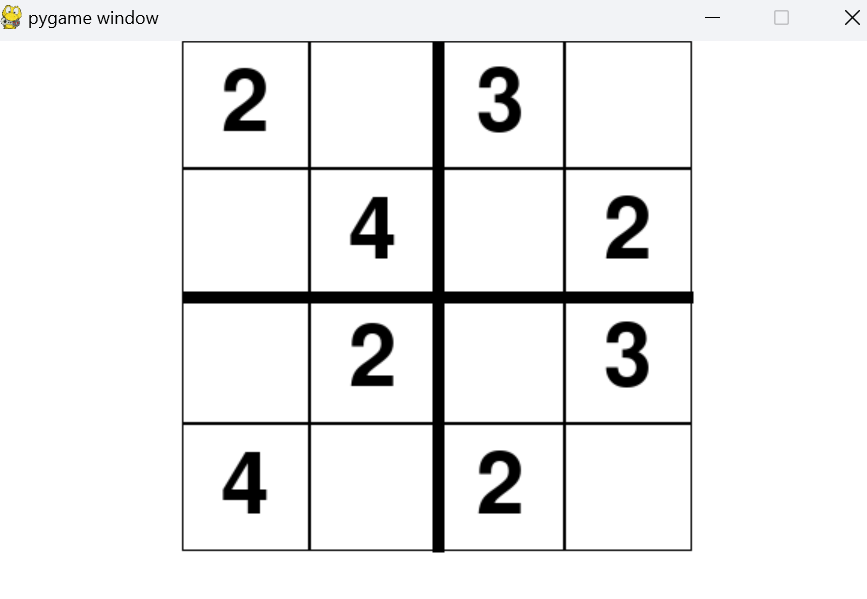
\includegraphics[width=\textwidth]{images/2x2 unsolved.png} 
        \caption{2x2 grid} 
        \label{fig:unsolved 2x2} 
    \end{minipage} 
    \hfill 
    \begin{minipage}{0.3\textwidth} 
        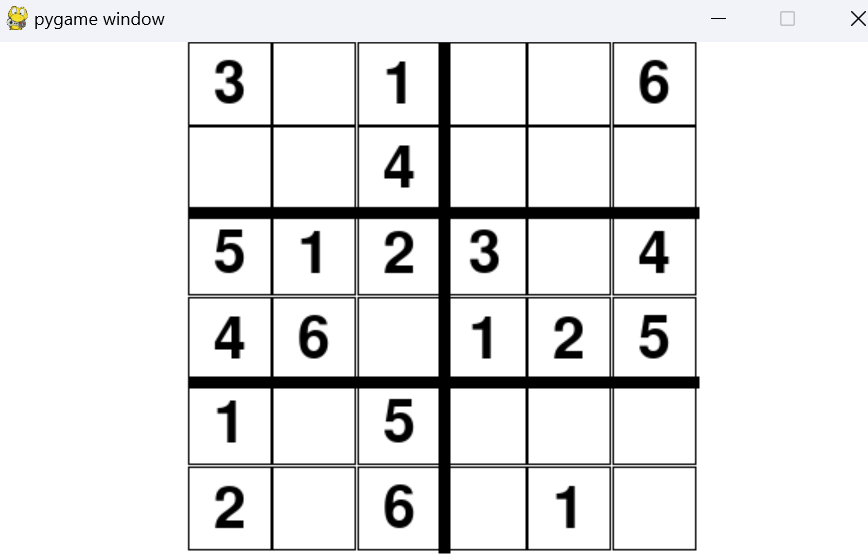
\includegraphics[width=\textwidth]{images/6x6 unsolved.png} 
        \caption{6x6 grid} 
        \label{fig:unsolved 6x6} 
    \end{minipage} 
    \hfill 
    \begin{minipage}{0.3\textwidth} 
        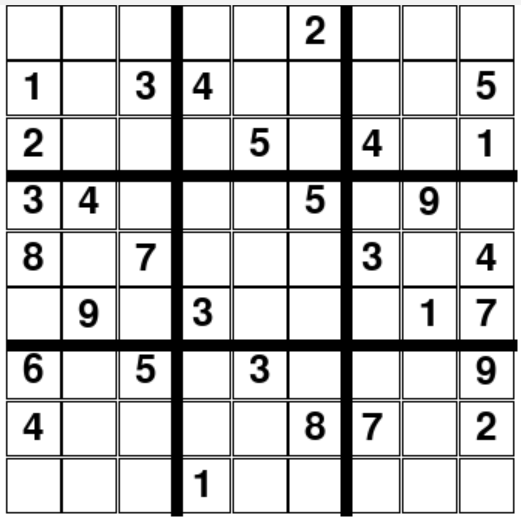
\includegraphics[width=\textwidth]{images/9x9 unsolved.png} 
        \caption{9x9 grid} 
        \label{fig:unsolved 9x9} 
    \end{minipage}
    \begin{minipage}{0.3\textwidth} 
        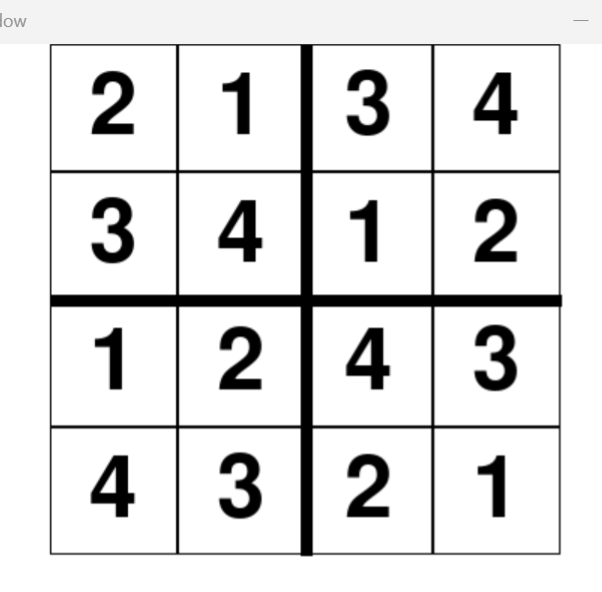
\includegraphics[width=\textwidth]{images/2x2 solved.png} 
        \caption{2x2 grid} 
        \label{fig:solved 2x2} 
    \end{minipage} 
    \hfill 
    \begin{minipage}{0.3\textwidth} 
        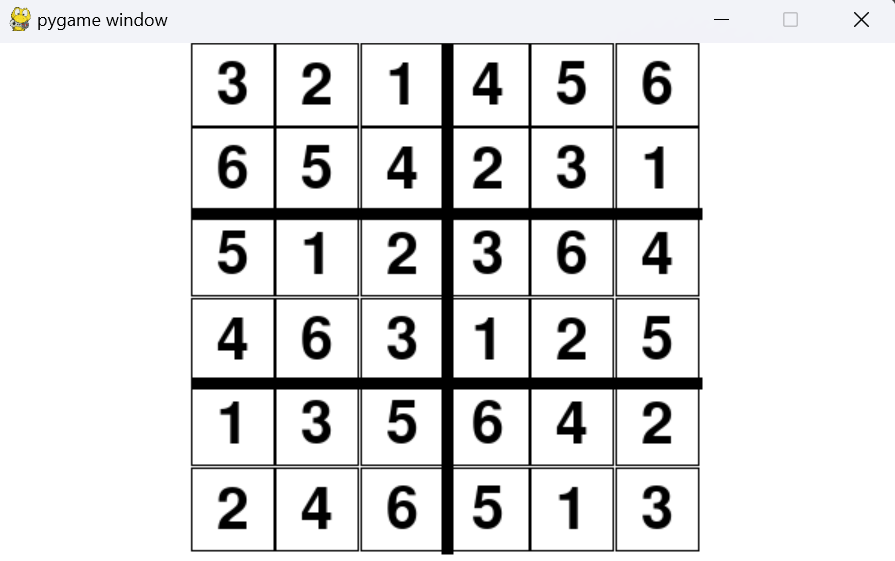
\includegraphics[width=\textwidth]{images/6x6 solved.png} 
        \caption{6x6 grid} 
        \label{fig:solved 6x6} 
    \end{minipage} 
    \hfill 
    \begin{minipage}{0.3\textwidth} 
        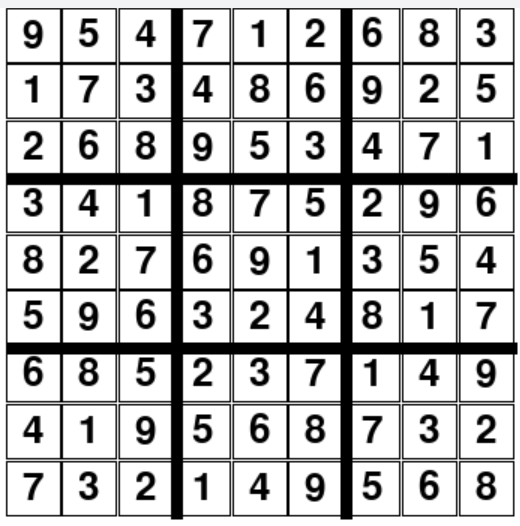
\includegraphics[width=\textwidth]{images/9x9 solved.png} 
        \caption{9x9 grid} 
        \label{fig:solved 9x9} 
    \end{minipage}
\end{figure}

%%%%%%%%%%%%%%%%%%%%%%
%%% Next Obectives
\chapter{Next Objectives}

\section{Development of Neural Network solution}
\subsection{What is a Neural Network?}

A neural network is based off of how the humans are capable of thinking through the use of a network of interconnected neurons. A neural network mimics the human brain’s neuron connections through modelling an interconnected network of nodes which can receive information, process the data and output that data either to another layer in order to attempt a greater accuracy in its prediction through additional processing, or to the user as a final prediction output \cite{Dongare2012}. the model is capable of learning from its mistakes through the use of backpropagation and can also process information in parallel all of which can help the model to do things like pattern recognition, which can be applied to many different fields and problems which could potentially be the best means of finding a solution \cite{Woodford2023}. 

This Artificial Intelligence model is implemented by separating the interconnected network into layers. These layers are the input layer, the hidden layer (or layers) and the output layer \cite{IBM2024} . The input layer is the primary layer that is used to take in all the inputs to be processed, hence its name. The hidden layers consist of the nodes that begin to process the inputted data, this is done through weights and biases associated with the connection between 2 nodes. These nodes are trained through passing in test data to help set and adjust the weights and biases of the connected nodes, by using a technique called backpropagation the algorithm can analyse predicted outputs and based on the output, make changes to weights and biases to update model and reduce its rate of error, allowing for growth and the ability to learn from its own mistakes \cite{Schmidhuber2015} . The output layer is responsible for compiling the final prediction to be used as a solution to the problem it was provided to solve. 

\subsection{How can this be Implemented into my Application?}

The next focus of the project moving forwards will be on developing a Neural Network that will be trained on taking in sudoku solutions, this is so that it will learn what a solution to a sudoku should look like and it should recognise the patterns/rules of a sudoku so that when it is faced against an incomplete sudoku, it will be able to provide an accurate prediction of a solution, that will hopefully be the correct answer to the inputted problem.

With the use of a neural network, there is a possibility of overfitting, which is when the network produces great results when working within the training data, but when introduced to a new puzzle outside of the training set, the algorithm holds poor results. This is a risk to consider when developing the AI sudoku solver as poor results will impact the validity of the project results which will need to be able to show the effectiveness of artificial intelligence when implementing it in an environment to play games and solve puzzles. To mitigate this risk, it would be important need to dedicate time in the next term to researching solutions to overfitting, such as pruning, cross validation or data augmentation. 

\section{Further Improvements planned for the GUI}

Once the other features of the project have become slightly more developed, the next planned step is to return to improve the sudoku interface through various means, such as randomised sudoku generation of varying difficultly, as well as making graphical changes to utilise components such as radio buttons or checkboxes to select which algorithm to use when solving the puzzle, also implementing a reset button to clear the grid and a start button to start the algorithm would help to make the application experience more user friendly and convenient. Additional text would also be needed, and useful for displaying the time it takes for solving the problem as well as potentially a mistakes counter for how efficiently/accurately it initially solves the problem.

\section{Next Term Timeline}

Time at the end of the term will need to be spent on the compiling all the work done in the project so that a full application and full report can be produced, presented and submitted, so the amount of time that can be allocated on the development of the AI sudoku solver is limited, however with this limited time the project can be completed to a suitable degree, and the plan for how this will be accomplished is listed below:

\begin{itemize} 
    \item \textbf{Weeks 1-6:} Within the first 6 weeks of development, there should be significant progress made on the neural network model. The first 2 week would be spent on researching in more depth how I would begin to tackle this problem, but the following weeks would need to be spent programming the algorithms needed to build the model and significant time will be focused testing the model with training data so that the sudoku solver will be able to output proper and accurate predicted solutions to the presented problems the user may want to pass in.

    \item \textbf{Weeks 6-8:} The following 2 weeks will be spent on updating the programmed AI solving algorithms so that the algorithms are able to monitor its own statistics so that the interface can display its results when solving a sudoku. These stats should show the speeds that the algorithm takes to solve the passed in problem, and the number of mistakes it took for it to get the final, valid solution to the problem. This feature would be a focal point as it is necessary to show how well the algorithms tackle these problems and prove its intelligence. 
    
    \item \textbf{Weeks 8-10:} The final few weeks of development will be spent on improving overall user experience and optimising the solving algorithms so that in the end of development a final, polished product is produced, with very little to no bugs and a very user friendly display features with super fast artificial intelligence algorithms that are capable of solving any sudoku with a solution, presented to it. 
\end{itemize}

%%%%%%%%%%%%%%%%%%%%%%
%%% conclusion
\chapter{Conclusion}

In conclusion, the development of the AI sudoku solver has been coming along well as sighnificant progress has been made and milestones such as the development of the console interface, the graphical user interface and the Backtracking solving algorithm itself, which was the first planned AI algorithm to be implemented, has been achieved which helps the application to demonstrate how Artificial intelligence is superior to human intelligence due to its computational capacities and speed and how it can be applied and adapted to a gaming environment, in order to attempt to play games and solve puzzles efficiently through learning from its mistakes and finding a valid solution for a problem, which in the case of this project, is a solution to different sudokus of various sizes and difficulty. 

With the next term of development, the areas of focus for the Artificial Intelligence sudoku solver will be the development of the Neural network model, displaying algorithm statistics in order to provide metrics which can be used to back up and prove the claims made by this project, as well as further improving the user interface so that the application as a whole will be more user friendly and easy to work with so that my points can be more effectively monitored  and displayed in a more digestible manner. 

%%%% ADD YOUR BIBLIOGRAPHY HERE
\newpage
\begin{thebibliography}{99}
\addcontentsline{toc}{chapter}{Bibliography}

\bibitem{AIforSocialGood} 
AI for Social Good (n.d.). Artificial Intelligence vs. Human Intelligence: Exploring the Debate and Key Points. [online] Available at: \url{https://aiforsocialgood.ca/blog/artificial-intelligence-vs-human-intelligence-exploring-the-debate-and-key-points} [Accessed 8 Oct. 2024].

\bibitem{Strachey1952} C. Strachey, Logical or non-mathematical programmes, in: Proc. Association for Computing Machinery Meeting, Toronto, ON, 1952, pp. 46–49.

\bibitem{Kister1957} J. Kister, P. Stein, S. Ulam, W. Walden, M. Wells, Experiments in chess, J. ACM 4 (1957) 174–177.

\bibitem{GeeksforGeeks} GeeksforGeeks (n.d.). Sudoku | Backtracking-7. [online] Available at: \url{https://www.geeksforgeeks.org/sudoku-backtracking-7/} [Accessed 9 Oct. 2024]. 

\bibitem{AkinDavid} Charles Akin-David, Richard Mantey, n.d. Solving Sudoku with Neural Networks. [pdf] Available at: \url{https://cs230.stanford.edu/files_winter_2018/projects/6939771.pdf} [Accessed 10 Oct. 2024].

\bibitem{Brailsford1999} S. C. Brailsford, C. N. Potts, and B. M. Smith, \textit{Constraint satisfaction problems: Algorithms and applications}, European Journal of Operational Research, vol. 119, no. 3, pp. 557-581, 1999. Available at: \url{https://www.sciencedirect.com/science/article/abs/pii/S0377221798003646}

\bibitem{vanBeek2006} P. van Beek, \textit{Backtracking Search Algorithms}, Foundations of Artificial Intelligence, vol. 2, pp. 85-134, 2006. Available at: \url{https://www.sciencedirect.com/science/article/abs/pii/S1574652606800088}

\bibitem{Melanie2024} Melanie, \textit{Backtracking: What is it? How do I use it?}, DataScientest, 29 Mar 2024. Available at: \url{https://datascientest.com/en/backtracking-what-is-it-how-do-i-use-it}

\bibitem{Dongare2012} A. D. Dongare, R. R. Kharde, and A. D. Kachare, \textit{Introduction to Artificial Neural Network}, International Journal of Engineering and Innovative Technology (IJEIT), vol. 2, no. 1, pp. 189-194, 2012. Available at: \url{https://citeseerx.ist.psu.edu/document?repid=rep1&type=pdf&doi=04d0b6952a4f0c7203577afc9476c2fcab2cba06} 

\bibitem{Woodford2023} C. Woodford, \textit{How neural networks work - A simple introduction}, Explain that Stuff, 12 May 2023. Available at: \url{https://www.explainthatstuff.com/introduction-to-neural-networks.html} 

\bibitem{IBM2024} IBM, \textit{What is a Neural Network?}, IBM, 2024. Available at: \url{https://www.ibm.com/topics/neural-networks} 

\bibitem{Schmidhuber2015} J. Schmidhuber, \textit{Deep Learning in Neural Networks: An Overview}, Neural Networks, vol. 61, pp. 85-117, 2015. Available at: \url{https://arxiv.org/abs/1404.7828}

\end{thebibliography}
\label{endpage}

\chapter*{Appendix}
\addcontentsline{toc}{chapter}{Appendix}
\subsection*{Sudoku Interface}

\subsubsection{Importance of Interface Implementation}

The main focus for the start of my project needs to be the interface for displaying the sudoku. this is a necessary starting point as in order to demonstrate Artificial Intelligence solving the sudoku, my product needs to be able to display both the unsolved and solved solution in a way that is easily digested by the target audience. the borders, regions, numbers and void values need to be distinct and observable to those trying to understand what the AI algorithms is trying to achieve, and if the algorithms are doing so correctly. that makes this element of the product integral to the development of my project. 

\subsubsection{Implementation of Sudoku Interface}

In order to implement this feature, I have decided to initially work on a console based interface. I felt this was necessary as my first iteration of the sudoku interface only needs to display an easily readable representation of the sudoku puzzle. this was achievable in the console as the borders can be represented through the '-' character for row division and '|' character for column division, the numbers as just numbers and the void values as an '*' character. this gave a simple and easy to read sudoku display on the console. 

\subsubsection{Planned Improvements to the Interface} 

Once the other features of my project have become slightly more developed, I plan to return to improve the sudoku interface through various means, such as randomised sudoku generation of varying difficultly, as well as a better user interface to display the sudoku rather than primarily using the console, which works well and is readable, but is not the best means of displaying the puzzle in a visually appealing and user friendly fashion. 

\subsection*{Solving Algorithm} 

\subsubsection{How a Backtracking Algorithm could Solve a Sudoku} 

A backtracking works similar to how a human would back track. The algorithms makes an attempt to solve a problem. so in the case of a sudoku it would attempt to fill in blank squares with a potential solution, and when a problem occurs in its solution, it goes back to the cause of the problem, which would be the invalid potential solution in that square or a previous one, and continues its attempt with a different solution for the sudoku, and this is done repeatedly till a viable solution is formed.  

\subsubsection{Implementation of Backtracking Algorithm} 

When developing the solving algorithm, first came the crucial element of finding a blank square in the grid, this would be represented by a 0 in the sudoku grid array. the coordinates on the grid would be returned to the main algorithm when found, then using these, the main loop will attempt to fill the square with numbers ranging from 1 to the max value, which is also the length of the grid (usually 9), until a viable value for the square is found (a value that is not repeated in the row, column or sub-grid). if a viable value cannot be found, the algorithm clears the current square and backtracks to the previous square, and checks the next values for viability, if there are no viable values, the algorithm will clear the current square and backtrack once again to the square before and once again try different values until a different viable value is found and the algorithm searches for the next blank value and the algorithm repeats itself, until there is no more blank squares, or no more values to try on the grid that gives a solution to the problem. 

\subsubsection{Planned Improvements for the Backtracking Algorithm} 

In order to improve the speeds of my backtracking algorithm, I would need to look into my uses of exhaustive searches which is used a lot in my algorithm for different functionalities such as, finding an empty square by looping through every value in the grid array, checking validity of a value by searching through every value in the row, column and sub-grid for a repeated value. this is very inefficient, and I believe this can be rectified by maybe implementing faster search algorithms or making use of other methods and techniques to make the searches slightly quicker and efficient, which is necessary to prove AI's superior problem solving capabilities. 

\subsection*{Improvement of the User Interface}

\subsubsection{Creating a Graphical User Interface} 

When creating my graphical user interface to display the sudoku and the solving algorithm, I decided to pygame as it provides an adaptable environment in which the sudoku grid can be drawn on the window and updated with little difficulty while still being able to display a way of visualising the backtracking algorithm. when creating the grid, I decided to give it the length 340 which was big enough for the user to see the sudoku and the values in each square clearly. When dividing the grid into sub-grids I used the same divisor logic used in the console print function, however I divided the grid visually using thicker lines to create the division between the whole and sub grids. I then started adding values to square by placing a new square over the empty square with the intended value, this could be cleared through overwriting the square by filling the surface with a white square then updating the value to a new square to cover the cleared square. this function would need to be called every time the value changed in the algorithm in order to give the visual backtracking effect. 

\subsubsection{The Benefits of Having a GUI to Display the Problem Solving Algorithm} 

By introducing a GUI to display the solving algorithm, I am able to show the step by step solution being formed through mistake adaptation approach my backtracking algorithm takes as well as showing how quickly the computer can calculate this as the GUI updates the values very rapidly, demonstrating how much faster a computer is compared to a human, despite the GUI technically wasting computer processing speed, so it is faster to print the output directly then updating a GUI, but then the algorithm will not be demonstrated in an easily comprehensible manner. 

\subsubsection{Planned Improvements to the GUI} 

In order to improve the Graphical User Interface I plan to make use of radio buttons or checkboxes to select which algorithm to use when solving the puzzle, I also feel a reset button to clear the grid and start button to start the algorithm would also be a nice touch, and will make the application experience more convenient. Additional text would also be needed, and useful for displaying the time it takes for solving the problem as well as potentially a mistakes counter for how efficiently/accurately it initially solves the problem. 

\subsection*{Next Solving Algorithm} 

\subsubsection{How could a Neural Network Solve a Sudoku} 

My focus moving forwards will be on developing a Neural Network that will be trained on taking in sudoku solutions, this is so that it will learn what a solution to a sudoku should look like and it should recognise the patterns/rules of a sudoku so that when it is faced against an incomplete sudoku, it will be able to provide an accurate prediction of a solution, that will hopefully be the correct answer to the inputted problem.

\end{document}

\end{article}
